\chapter{Astronomy with Gamma Rays}

\section{The Field of Astroparticle Physics}

The balloon flights of Victor Hess in 1912 \cite{Hess:1912srp} are
often times cited as the starting point of astroparticle physics,
because they gave reason to believe, that the measured ionizing
radiation is of extraterrestrial origin. 

In the following years, the radiation was referenced as \enquote{Höhenstrahlung} 
(see e.g. \cite{myssowsky1926versuche}) 
and \enquote{cosmic rays} (see e.g. \cite{millikan1928origin}) with 
the english term cosmic rays eventually winning out.

Later, in 1933, Carl D. Anderson discovered the existence
of antimatter using a cloud chamber \cite{PhysRev.43.491},
which is crucial for the measurement of especially
high energy photons.

More research brought the discovery of several new particles,
that are imperative to modern gamma-ray astronomy:
pions \cite{LATTES1947}, muons \cite{PhysRev.52.1003}
and neutrinos \cite{Cowan103}.

Recently, the so far last discovery on this journey
was made with the measurement of the first gravitational 
waves \cite{PhysRevLett.118.221101}.

This leaves the field of astronomy with four different
messengers:
\begin{enumerate}
	\item Electromagnetic radiation
	\item Cosmic rays
	\item Neutrinos
	\item Gravitational waves
\end{enumerate}

Figure \ref{fig:multi_messenger} illustrates the key differences between
photons, hadrons and neutrinos.
This thesis focuses on the detection of cosmic and gamma rays.

\begin{figure}
	\centering
	\captionsetup{width=0.9\linewidth}
	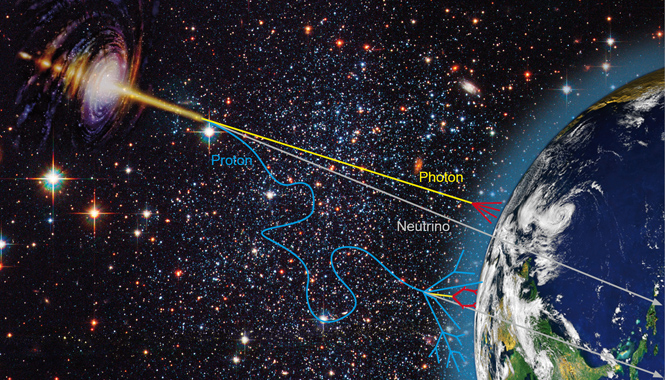
\includegraphics[width=0.8\textwidth]{images/astro-web-titel.jpg}
	\caption{Visualization of the behaviors of different messenger
		particles in modern astronomy.
		Photons and neutrinos travel through the universe without deflection,
		because they do not carry an electric charge.
		Neutrinos interact less than photons in the universe, the atmosphere and 
		the detecting experiments.
		Cosmic rays are deflected by interstellar
		magnetic fields and thus generally do not allow for a reconstruction
		of the source position \cite{desy_mm_astro}.
	}
	\label{fig:multi_messenger}
\end{figure}

In contrast to charged cosmic rays, gamma rays point towards
their sources, allowing to search for sources of radiation.
This makes it possible to learn more about the acceleration processes
and the sources, that produce high energy gamma and cosmic rays.
Two important classes of proposed sources are active galactic nuclei,
which are considered to be powered by super massive black holes, and 
supernova remnants. The best known example for a supernova remnant
is the Crab Nebula \cite{1989ApJ...342..379W}.
Due to its high and constant flux in the gamma-ray regime,
it is often times used as a \enquote{standard candle} to compare experiments and
analyses.

Researching the diffuse component of gamma rays on the other hand holds
potential to find out more about interstellar magnetic fields and the
propagation of relativistic particles in the universe.

Another motivation to research gamma rays lies in the assumption, that
dark matter could annihilate into photon pairs \cite{Weniger_2012}.

Due to the way gamma rays are being detected, it is generally impossible
to avoid measuring cosmic rays as well.
At the same time cosmic rays are much more numerous,
which usually makes them the dominant background in gamma-ray 
astronomy \cite{funcray}.

\section{Production of Gamma Rays}
Creation of high-energy gamma rays cannot happen thermally,
but occurs in a combination of high energy charged particles 
and interstellar targets or magnetic fields \cite{funcray}.
A model for the production at the source, the Self Synchrotron Compton model,
focuses on photon emission from an initial pure electron distribution.
The key aspects of this model are now briefly presented. 

\newpage
\textbf{Synchrotron Radiation}

Proposed sources of cosmic rays and gamma-rays include 
high magnetic fields. Any moving charged particle will thus be
deflected perpendicular to its moving direction
due to the Lorentz force, forcing them on a radial trajectory.
At the same time, a relativistic charged particle, 
that is accelerated radially, emits synchrotron 
photons. The emitted power is

\begin{equation}
	P \propto \frac{1}{m^4} \left(E^2 - m^2c^4\right)^2.
	%\langle E_{\gamma} \rangle \propto \frac{1}{M_P} E_P^2 B^2.
	\label{eq:synchrotron}
\end{equation}

Here, $m$ and $E$ denote the accelerated particle's 
mass and energy respectively. %With this %the inverse mass dependency
With hadronic particles being much heavier than electrons
it is immediately evident that
synchrotron radiation plays a major role in leptonic 
emission and much less in hadronic emission.

A direct result of this is, that the electrons energy is reduced
in the process, affecting (\enquote{cooling}) the initial electron distribution.
This is sometimes referred to as synchrotron cooling.

The emitted synchrotron spectrum needs to be further modified,
if the emitting region is optically thick and photons 
are absorbed by the medium.
This is in fact always the case, as the regions contain
both magnetic fields and a high density of electrons.

\textbf{Inverse Compton Scattering}

In a classical particle interpretation photons and electrons 
can collide, exchanging energy and altering their directions.
For the normal case of Compton scattering, the electron 
is assumed to be at rest and the photon can never gain 
energy by colliding with the electron.
This is evident from the change of wavelength in \eqref{eq:compton},
with $\lambda^{\prime}$ the scattered photon's 
wavelength, $\lambda$ the initial photon's wavelength  
and $\Theta$ the scattering angle.

\begin{equation}
	\Delta \lambda = (\lambda^{\prime} - \lambda)  \propto \left(1-\cos{\Theta} \right)
	\label{eq:compton}
\end{equation}

If the electron itself is moving with much higher energy
than the photon, this changes and the photon can gain substantial energy.
This is referred to as inverse Compton scattering.
In that case transforming the equations to the 
electron's frame of reference and back to the laboratory frame of reference each
boosts the photon's energy by a factor proportional to 
the Lorentz factor of the electron.

For low energies, the cross section can be approximated by 
the Thomson cross section. 
When the photon energy and the rest energy of the electron
become comparable, the Klein-Nishina cross section has to be applied,
which is inversely proportional to the photon's
wavelength.
This, in turn with the energy transfer not increasing anymore at high energies,
suppresses the generation of high energy photons \cite{Nakar_2009} and
thus limits the flux at very high energies.

The Synchrotron Self Compton model combines the above mentioned
effects to produce a photon energy distribution from an initial
electron distribution, which is often times assumed to
follow a (broken) power-law or log-parabolic spectrum.
The free parameters of the model can be interpreted as 
three frequencies: The minimum injection frequency $\nu_m$,
the cooling frequency $\nu_c$ and the self-absorption frequency $\nu_a$.
Depending on the order of these parameters, different
photon distributions can be generated.

A detailed analysis of the influence of the parameters of
the Synchrotron Self Compton model, can be found in 
\cite{10.1093/mnras/stt1461}.

Calculations for the Synchrotron Self Compton model for a source
with an age of 1000 years, a magnetic field of
\SI{100}{\micro\gauss} and a initial electron spectrum, that
follows a power-law with index $\Gamma=2$ before cooling and 
$\Gamma=3$ after cooling, can be seen in figure \ref{fig:sct_model}.
The photon distribution shows two peaks due to the
two relevant processes.
The flux at energies $\gg \SI{100}{\giga\electronvolt}$
falls off rapidly. Subsequently, experiments
observing at higher energies require large detector areas
to achieve relevant event counts.

\begin{figure}
	\centering
	\captionsetup{width=0.9\linewidth}
	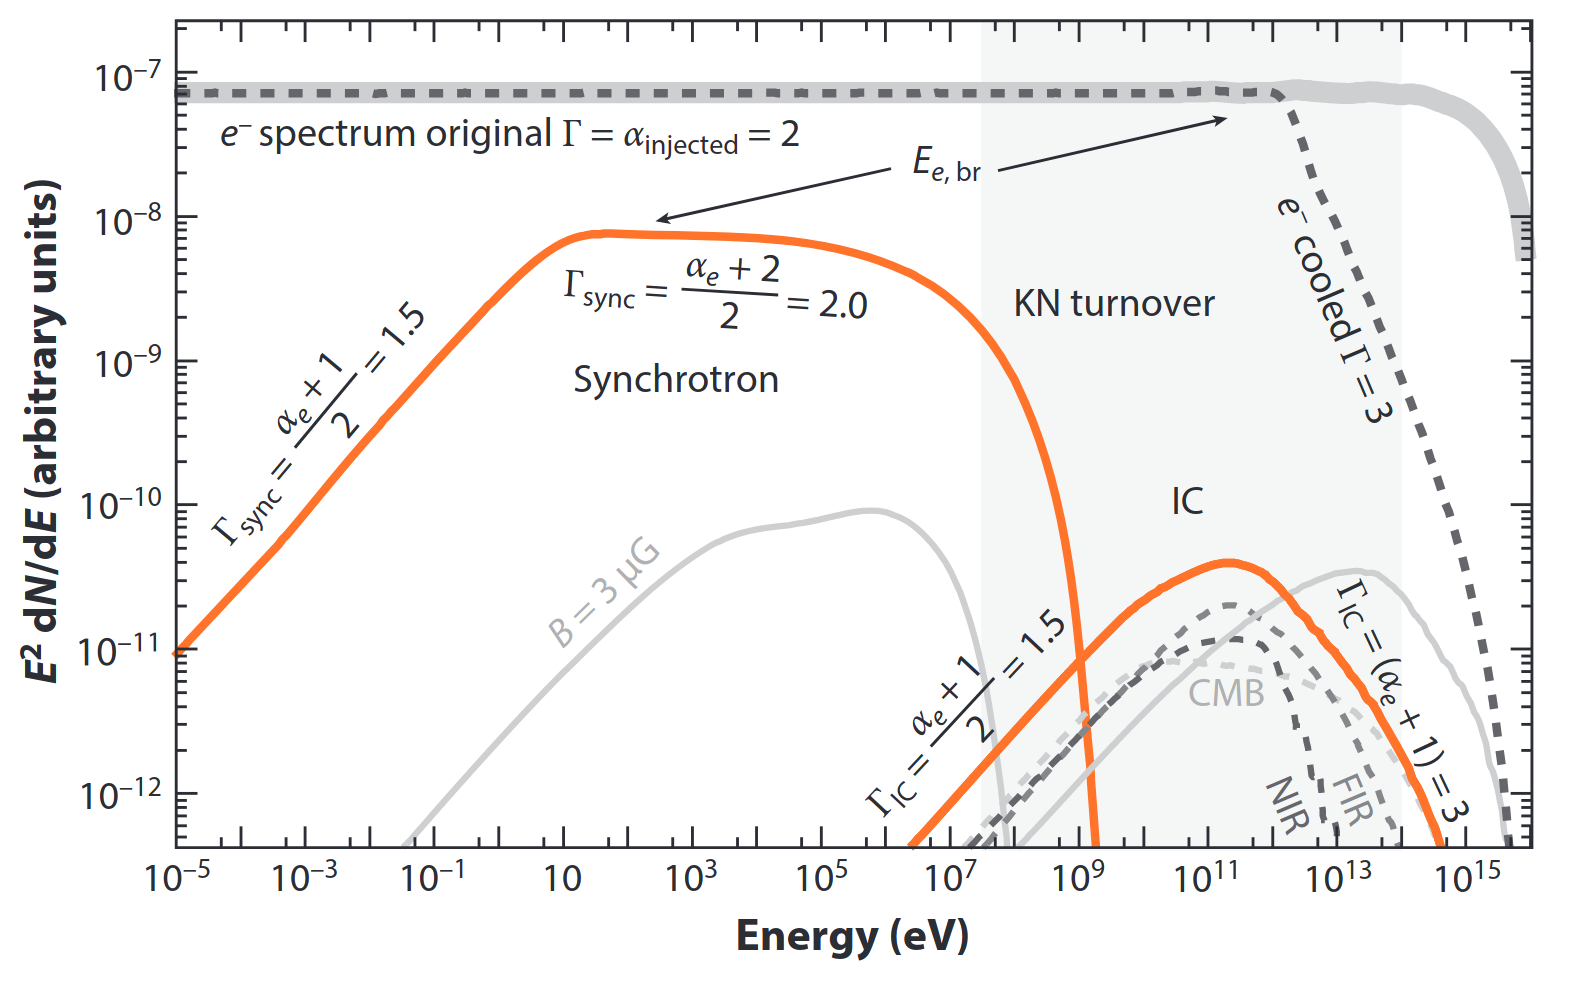
\includegraphics[width=0.8\textwidth]{images/sct_spectrum.png}
	\caption{Illustration of the spectral distribution of 
	the initial electrons (gray) and the accelerated photons (orange)
	in the Synchrotron Self Compton model.
	The 
	Two photon distributions are visible, one due to the synchrotron and one  
	due to the inverse compton effect \cite{funcray}.
	}
	\label{fig:sct_model}
\end{figure}



\section{Experiments for Cosmic and Gamma Rays}
Emitted gamma rays can be observed either directly
from outside the atmosphere via satellites or indirectly
via ground based gamma experiments.
If measuring below the atmosphere, the original particle
cannot be observed directly, because it interacts with the atmosphere
and produces secondary particles. This produces what is called an air shower.

The different types of experiments differ in the way particles are detected and
the energy ranges, in which they operate.

\subsection{Satellite Experiments}
Satellite experiments allow direct measurements of gamma and cosmic rays, because they operate
above the atmosphere.
This allows to use similar techniques as experiments located at terrestrial 
particle accelerators: Incoming photons hit an initial layer and produce an $e^+/e^-$-pair 
via pair production. The tracks of these particles are observed before they reach the calorimeter,
where their energies are measured.

Despite the advantages over ground based experiments, the small detector areas 
limit the sensitivities at higher energies.

A currently operating experiment is the FERMI Gamma-ray Space Observatory (FGST) \cite{Atwood_2009}.
The Large Area Telescope on 
the FGST covers an energy range of
\SI{20}{\mega\electronvolt} to \SI{100}{\giga\electronvolt} \cite{Atwood_2009}.
It is able to see in a huge field of view of 
\SI{2.4}{\steradian}. A second detector, the Gamma-ray Burst Monitor,
searches for gamma-ray bursts to notify other experiments.

\subsection{Imaging Air Cherenkov Telescopes}
A class of ground-based observatories are the 
Imaging Air Cherenkov Telescopes (IACTs),
which will be the main focus of this thesis.

In contrast to satellite experiments, they cannot directly
observe the cosmic particles. Instead they use the atmosphere as detector medium.
High energy primary particles generate a cascade of secondary particles
when interacting with the atmosphere. These particles generate cherenkov
light, which is recorded by the IACTs.
This allows for huge effective detector areas of the order of
multiple \si{\square\kilo\meter}.
Because the cherenkov light has the wavelength of visible light,
IACTs can only reasonably operate at nights with good conditions.

Modern experiments include 
MAGIC \cite{ALEKSIC2012435},
VERITAS \cite{WEEKES2002221}
and HESS \cite{vincent2005hess},
all of which consist of multiple telescopes to observe the showers
from different angles in order to improve the reconstruction.

The observable energy range generally generally lies in the range of
some \SI{10}{\giga\electronvolt} to some 10-\SI{100}{\tera\electronvolt}.

\subsection{Air Shower Arrays}
Air shower arrays, like IACTs, operate on the ground and thus also have 
to measure the particle indirectly.

In contrast to IACT-experiments, air shower arrays consist of a large
number of single scintillation detectors or photomultiplier tubes.
Instead of the cherenkov light, they measure the
remaining particles of the shower. This makes them feasible
for energies even above the ones measured by IACTs.
In addition, air shower arrays generally have a higher duty cycle than
IACTs, because they do not rely on optical light and therefore can operate
at nearly all days of the year.

A modern experiment is the High Altitude Water Cherenkov Observatory (HAWC) \cite{2015ICRC...34..966S}.
It uses \num{300} water tanks to measure air showers with a lower threshold
of under \SI{1}{\tera\electronvolt}.
